%!TeX root=../../master.tex
\section{Gesture Recognition}\label{sec:gesturerecognition}
The system lets users control smart devices in their home by performing certain gestures.

Gesture recognition can generally be split into two categories: 
Camera-based and motion-based \cite{Kela2006}. 
Examples of camera-based gesture recognition systems are the ``Gesture Pendant'' \cite{starner2000gesture} and the Kinect \cite{kinect}, 
and an example of a motion-based system is the Reemo \cite{Reemo}.

The camera-based solution require that the limbs, 
used to perform gestures, 
are visible to the camera, 
and as such \emph{static} cameras placed in a room, 
may be rendered useless if the user turns his back against them. 
In addition, furniture and other people may stand in between them, 
and obstruct the line of sight between the camera and the user.
This would likely not happen with the ``Gesture Pendant'', 
but the user would have to make sure that the pendant was always outside of any clothes worn, 
as putting on a sweater or wrapping yourself in a blanket, 
might block the view of the camera.

Motion-based solutions can employ various different sensors on the person,
such as accelerometers and gyroscopes, 
and depending on the type of sensor, 
different methods can be used to recognize gestures.
As mentioned in \Cref{sec:wearables}, accelerometers are present in about half of the wearables. 
Because of this, we will focus on finding a solution using accelerometer, 
so that we do not have to use additional hardware, such as cameras. 

In the following section, we will describe a gesture recognition system called the \$3 Gesture Recognizer. 


\subsection{\$3 Gesture Recognizer}\label{sec:threedollar}
The \$3 Gesture Recognizer is a gesture recognition system, 
created by Sven Kratz and Michael Rohs, 
and is presented in the paper ``A \$3 Gesture Recognizer – Simple Gesture Recognition for Devices Equipped with 3D Acceleration Sensors'' \cite{threedollar}.

The system is based on the \$1 Recognizer by Wobrock \etal \cite{wobbrock2007gestures}, 
and adds the ability to detect three dimensional gestures, 
rather than being limited to two dimensional gestures.

Both of these systems are designed to be easy to use by anyone for fast prototyping of user interfaces, 
which makes them appropriate for use in this project.
The \$3 Gesture Recognizer, however, is better suited, 
as it is capable of recognizing more gestures because it utilizes three dimensional data.
This means that users have even more options for personalizing the gestures, 
that they will use to control their home with.

In addition, the \$3 Gesture Recognizer only requires the user to train a gesture about five times, 
before it can deliver adequate recognition rates. 
This provides a better experience for the user, 
as he does not need to spend much time training the system before he is able to use it.
Whenever a user trains a gesture, 
a new gesture trace is stored and associated with a gesture class. 
A gesture class that has been trained five times, 
has five gesture traces stored.

The way the \$3 Gesture Recognizer works, 
is by collecting data from a three-axis accelerometer, 
and from this it creates a gesture trace $T$, 
which consists of a set of candidate points. 
This is illustrated in \Cref{fig:onedollar-gesturetrace}.

The figure also shows that the gesture traces can contain a different number of points, 
when performing the same gesture at different speeds.
Because of this, the \$3 Gesture Recognizer \emph{resamples} $T$, 
so that it contains a fixed number of points. 
In \cite{threedollar}, the number of points $N$ is \num{150}, 
with equal distance between the points.
If $N$ is set to a lower value, then precision is lost. 
If $N$ is set to a higher value, then computational cost increases.
After resampling the points, 
$T$ is rotated in an attempt to correct for any rotational error, 
and finally it is scaled to fit inside of a cube of $100^3$ units, 
to compensate for the fact that may perform inconsistently sized gestures.

Once all of these transformations have been performed, 
the gesture trace is matched against all the training gestures. 
From these comparisons a scoring table is created, 
where each trained gesture is given a score, 
based on the distance between it and the input gesture trace. 
To reduce the amount of false positives, 
a scoring heuristic is utilized, 
which simply determines whether a score is above a threshold $\epsilon$.

\todo[author=Thalley]{We should include a description of how gestures are compared. What's the math behind it?}

\begin{figure}[!htb]
  \centering
  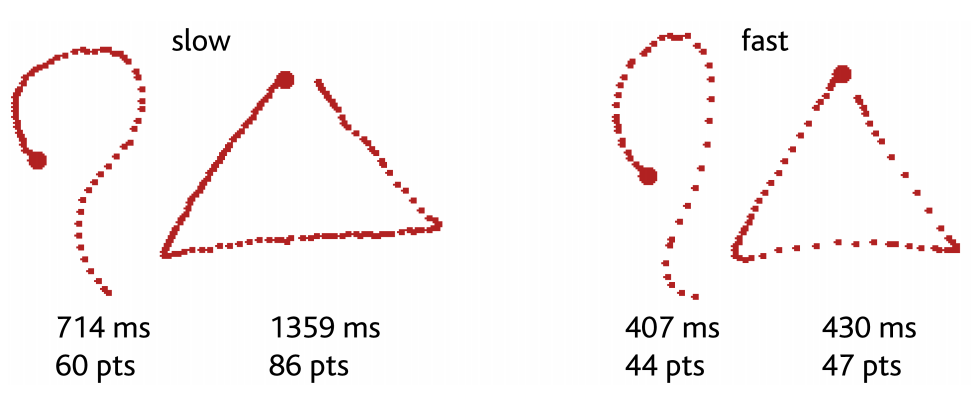
\includegraphics[width=0.8\textwidth]{images/1-dollar-gesturetrace.png}
  \caption{A slow and fast question mark and a triangle, made by subjects using a stylus on a Pocket PC. Note the considerable time differences and resulting numbers of points. Image and text is from Figure 3 in \cite{wobbrock2007gestures}}
  \label{fig:onedollar-gesturetrace}
\end{figure}

\subsection{Detecting Points Before and After Gestures}
Before a user performs a gesture in order to control an actuator, 
he must point at the actuator he desires to control. 
%Thalley: Describe the reason for this

A point is defined as the user holding his phone still for a small period of time. 
An accelerometer can be used to detect if the user holds the device still. 
If there is a low amount of activity on all three axes, 
it is assumed that the user is holding the device in his hand without moving it.

\Cref{fig:gesture-recognition:point-to-gesture-state-diagram} shows the relationship of a point and a gesture in a state diagram. 
All gestures begin and end with a point. 
When the first point is detected, 
a very short delay is introduced in order for the user to prepare to do the gesture, 
\eg move the position of his hand. 
%Thalley: Jeg kan ikke se hvorfor der skal være et delay. Kunne man ikke bare sige at man starter recognition så snart den ikke peger mere, efter at et peg at detected? 
The gesture recognition begins when the delay has passed. 
Gestures are recognized using the previously described \$3 Gesture Recognizer. 
After the gesture has been performed, 
the device must be held still again and the second point is detected. 
The collected gesture data is then analyzed by the \$3 Gesture Recognizer, 
in order to determine which known gesture was performed, if any at all. 
Lastly, the system returns to the initial state and another gesture can be performed.

While performing the gesture, the recognition may timeout. 
The \$3 Gesture Recognizer can recognize gestures for a maximum of four seconds before the recognition is canceled. 
In such case, the system returns to the initial state.

\begin{figure}[h]
\centering
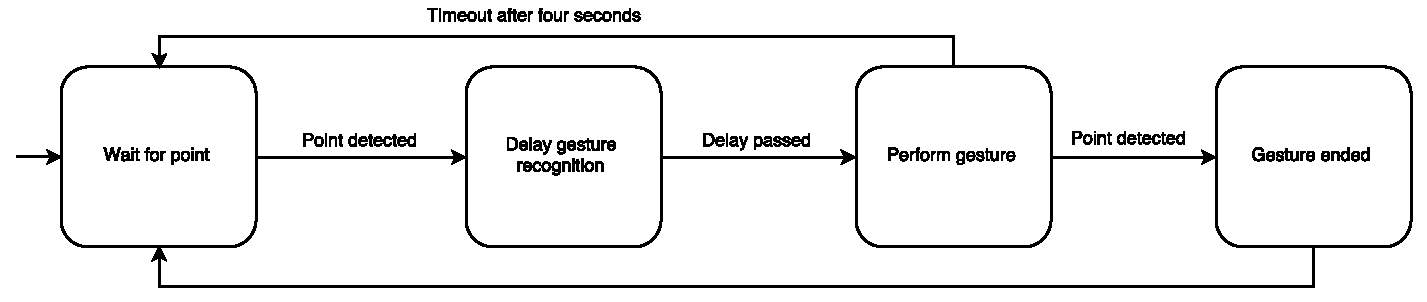
\includegraphics[width=\textwidth]{images/point-to-gesture-state-diagram}
\caption{State diagram showing the relationship between a point and a gesture. A gesture always starts and ends with a point.}
\label{fig:gesture-recognition:point-to-gesture-state-diagram}
\end{figure}

\subsubsection{Using Accelerometer Data to Detect a Point}

\Cref{fig:gesture-recognition:pointer} shows screenshots of an application, 
created to experiment with data from the accelerometer. 
The figure shows graphs of measurements made while the device was lying on a table (\Cref{fig:gesture-recognition:pointer:table}), 
the user was pointing with the device in his hand (\Cref{fig:gesture-recognition:pointer:hand}), 
and while the user was walking with the device in his hand (\Cref{fig:gesture-recognition:pointer:walk}).
We measure this so that we do not recognize a device laying still on a table, 
as a user pointing.
 
The $x$-, $y$- and $z$-values are measured in radians per second. 
The $y$-axis of the graph spans from \num{-5} to num{5}. 
The graphs shows that there are small, 
but measurable differences between the measurements made when the device is lying on the table,
and when the user is pointing with the device. 
This allows us to distinguish between the two scenarios, 
and disregard measurements made when the device is lying on the table. 

Furthermore the graphs clearly shows that there is a measurable difference between the values read when a user is pointing with a device, 
and walking with the device in his hand. 
Based on this small experiment, 
we can conclude that the accelerometer data can be used to determine if a user is pointing with a device.

\begin{figure}[!htb]%
    \centering
    \subbottom[Table]{\label{fig:gesture-recognition:pointer:table}
        \frame{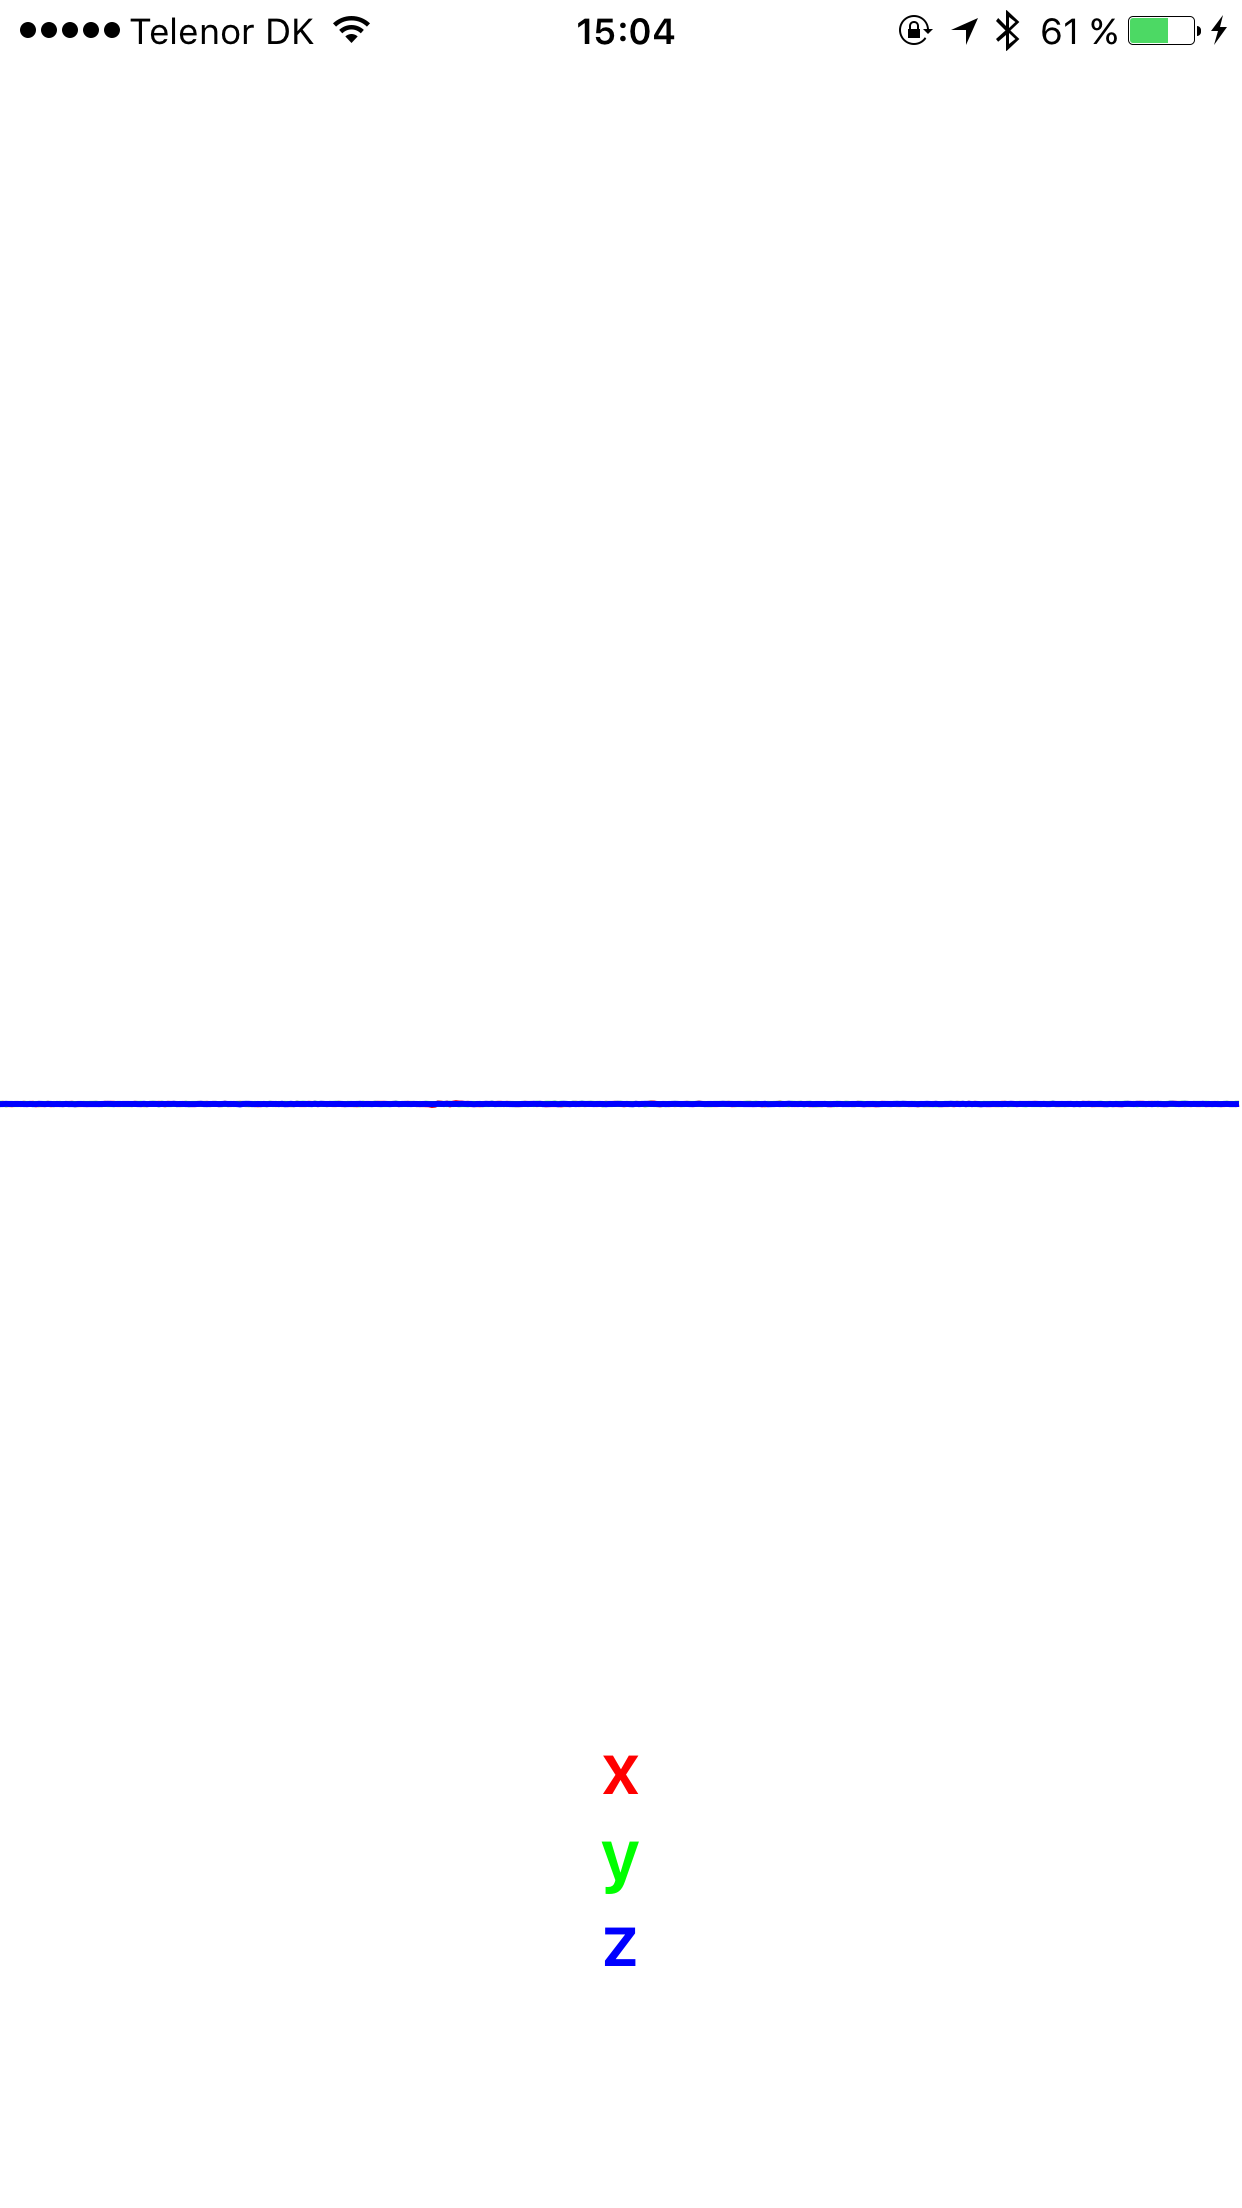
\includegraphics[width=0.3\textwidth]{images/pointer-table}}
    }
    \subbottom[Hand]{\label{fig:gesture-recognition:pointer:hand}
        \frame{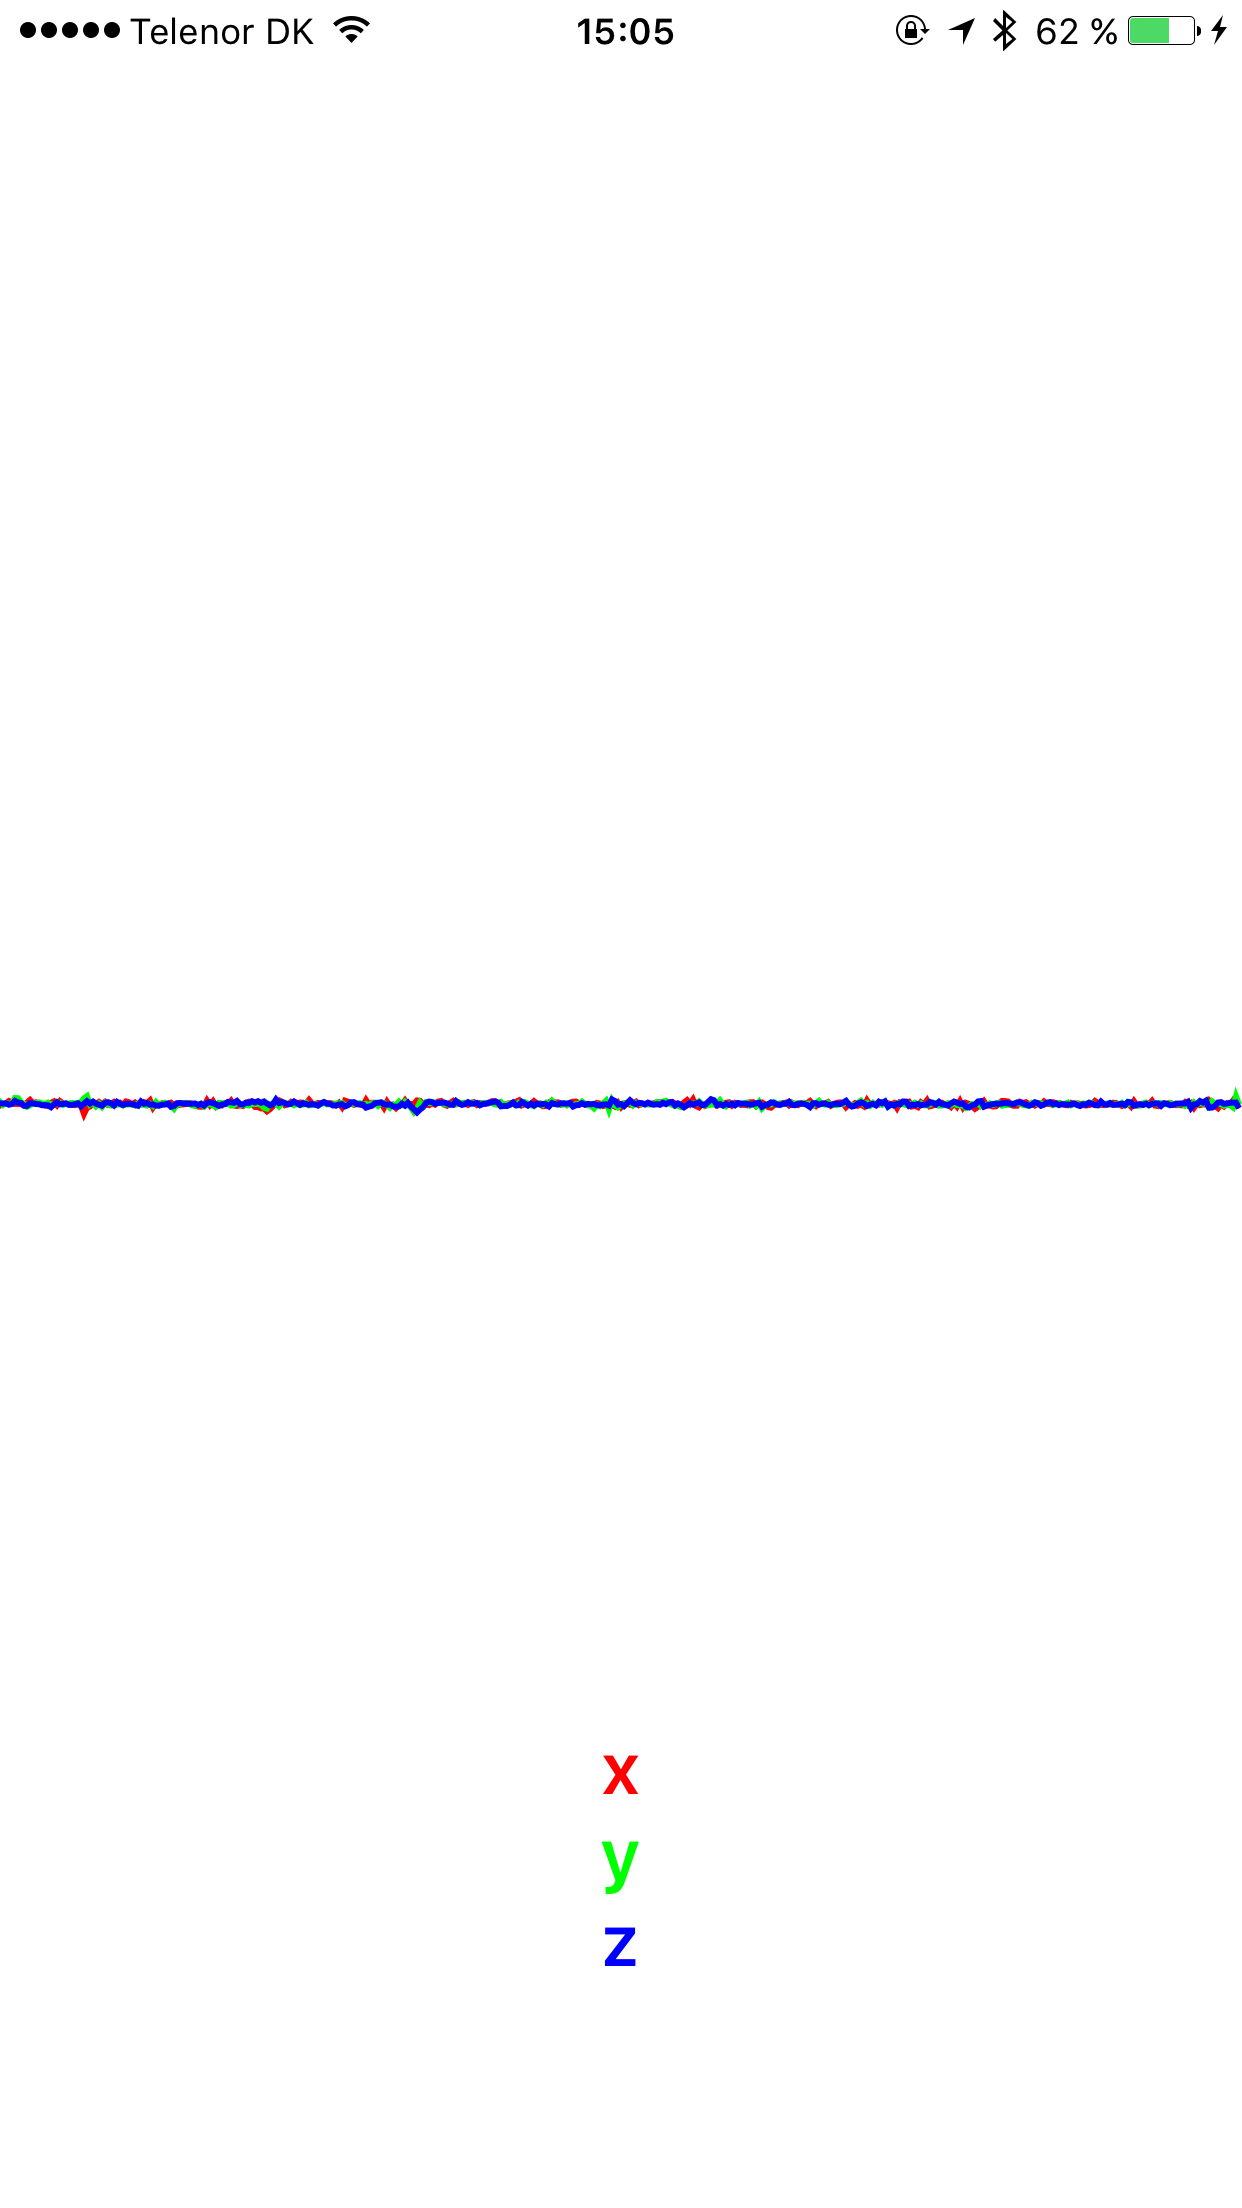
\includegraphics[width=0.3\textwidth]{images/pointer-hand}}
    }
    \subbottom[Walk]{\label{fig:gesture-recognition:pointer:walk}
        \frame{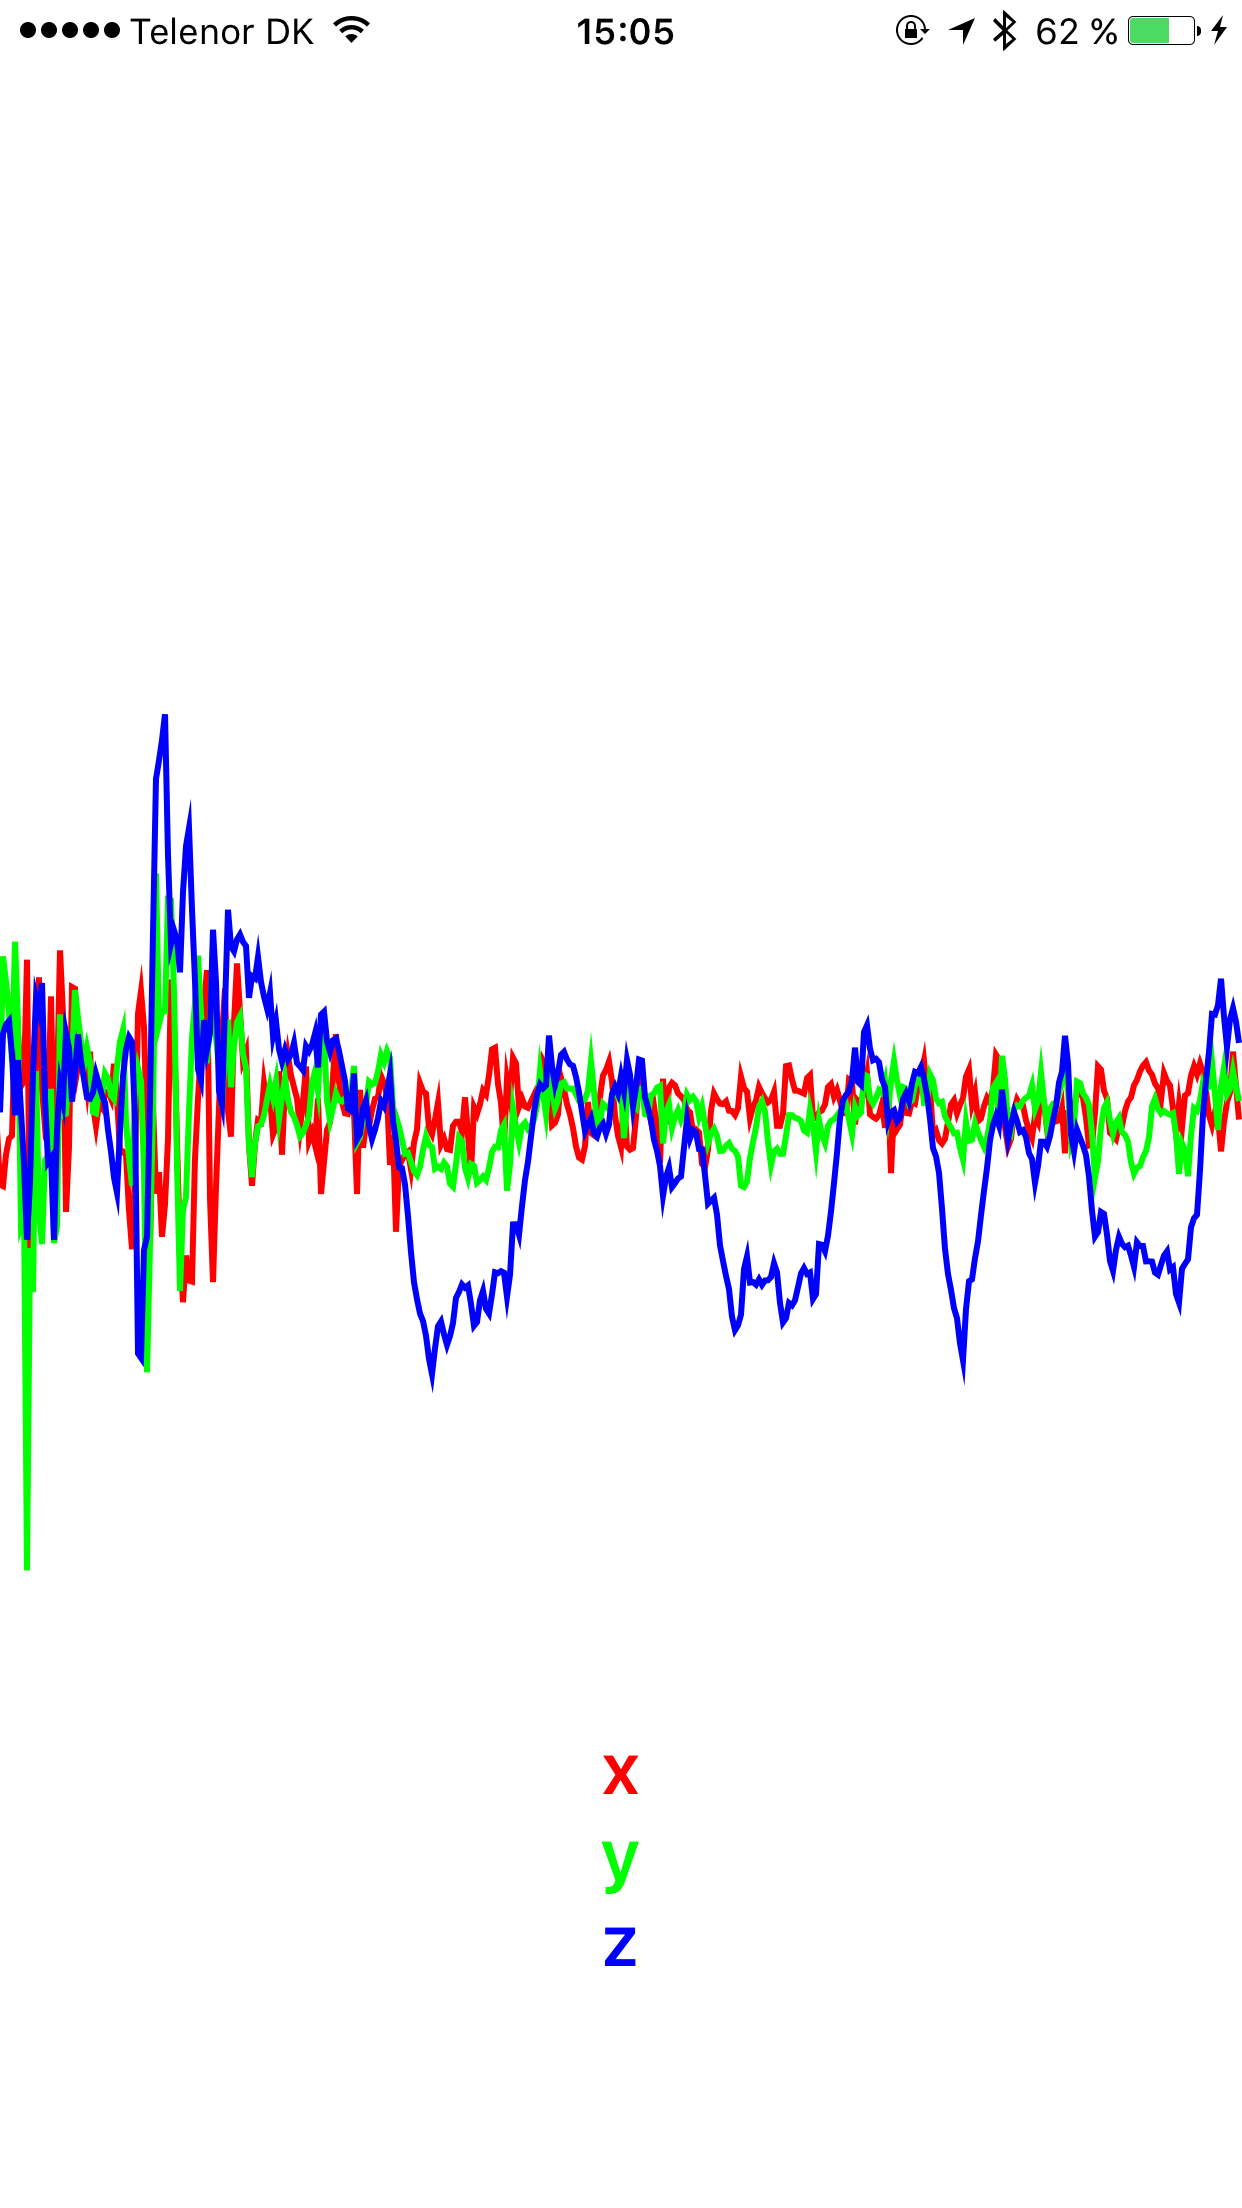
\includegraphics[width=0.3\textwidth]{images/pointer-walk}}
    }
    \caption{Screenshots of application created to experiment with data from the accelerometer. Leftmost screenshot shows graph of measurements made when the device lies on a table. The middle image shows graph of measurements made while pointing with the device. Rightmost screenshot shows graph of measurements made while the user was walking with the device in his hand.}
    \label{fig:gesture-recognition:pointer}
\end{figure}

\subsubsection{Detecting Points using PointDetector}

Part of the gesture recognition involves detecting if a user points. 
In order to limit the scope for the initial prototypes of the solution, 
we limit the context in which a point is detected, 
to a user walking with the phone in his hand, 
then stopping up to point at an actuator with the phone.

The \texttt{PointDetector} class receives data from the accelerometer data, 
and based on the data determines if a user points with the device. 
When a user points with the device, 
an instance of the class will inform a listener.

The state diagram in \Cref{fig:gesture-recognition:pointdetector-state-diagram} illustrates the internals of the \texttt{PointDetector} class. 
When instantiated, the object will not be detecting, 
\ie it will not be receiving accelerometer data. 
After the instantiation, the instance can begin detecting. 
The detection can be stopped at any time.

When detecting, the \texttt{PointDetector} will wait for the first set of data from the accelerometer, 
that indicates that the user is pointing. 
When the data is received, 
the object will enter the \textit{Sampling} state, 
in which it continuously checks data from the accelerometer, 
to determine if a set of data indicates a point. 
If the data indicates a point, 
both the \emph{point sample count} and the \emph{total sample count} will be incremented. 
If the data does not indicate a point, 
only the total sample count will be incremented.
%Thalley: Beskrivelse af de her sample counts bør nok ligge heroppe. Kunne ikke lige finde en pæn måde at gøre det på selv.

At the same time the detector enters the sampling state, 
it will start a timer that runs for a number of seconds. 
When the time has passed, 
the detector will leave the sampling state, 
and determine if the result of the sampling, 
indicates that the user is pointing. 

The sampling phase is necessary in order to avoid ``outliers'' in the data, 
\ie anomalies in the sensor data. 
The accelerometer continuously delivers data, 
and a single data set may indicate that the user is pointing. 
However, it may not be the users intention to point at all. 
It may be that he just held the device very still for a short moment.

In order to determine if the result of the sampling phase indicates a point, 
the detector investigates the relation between the point sample count, $p$, 
and the total sample count, $t$. 
If $p/t \geq c$, where $c$ is the necessary percentage of samples that must indicate a point, 
then the detector can conclude that the sample is indeed a point.

After the sampling phase has concluded, 
the detector will wait for a new data set from the accelerometer that indicates a point.

An accelerometer delivers an $x$-, $y$- and $z$-acceleration. 
Determining if a data set indicates a point is a matter of checking if the three values fits within some threshold, $h$. 
In order to check if the phone is lying still on a table, 
the values must be checked against another threshold, $g$. Note that $g < h$.

\begin{figure}
\centering
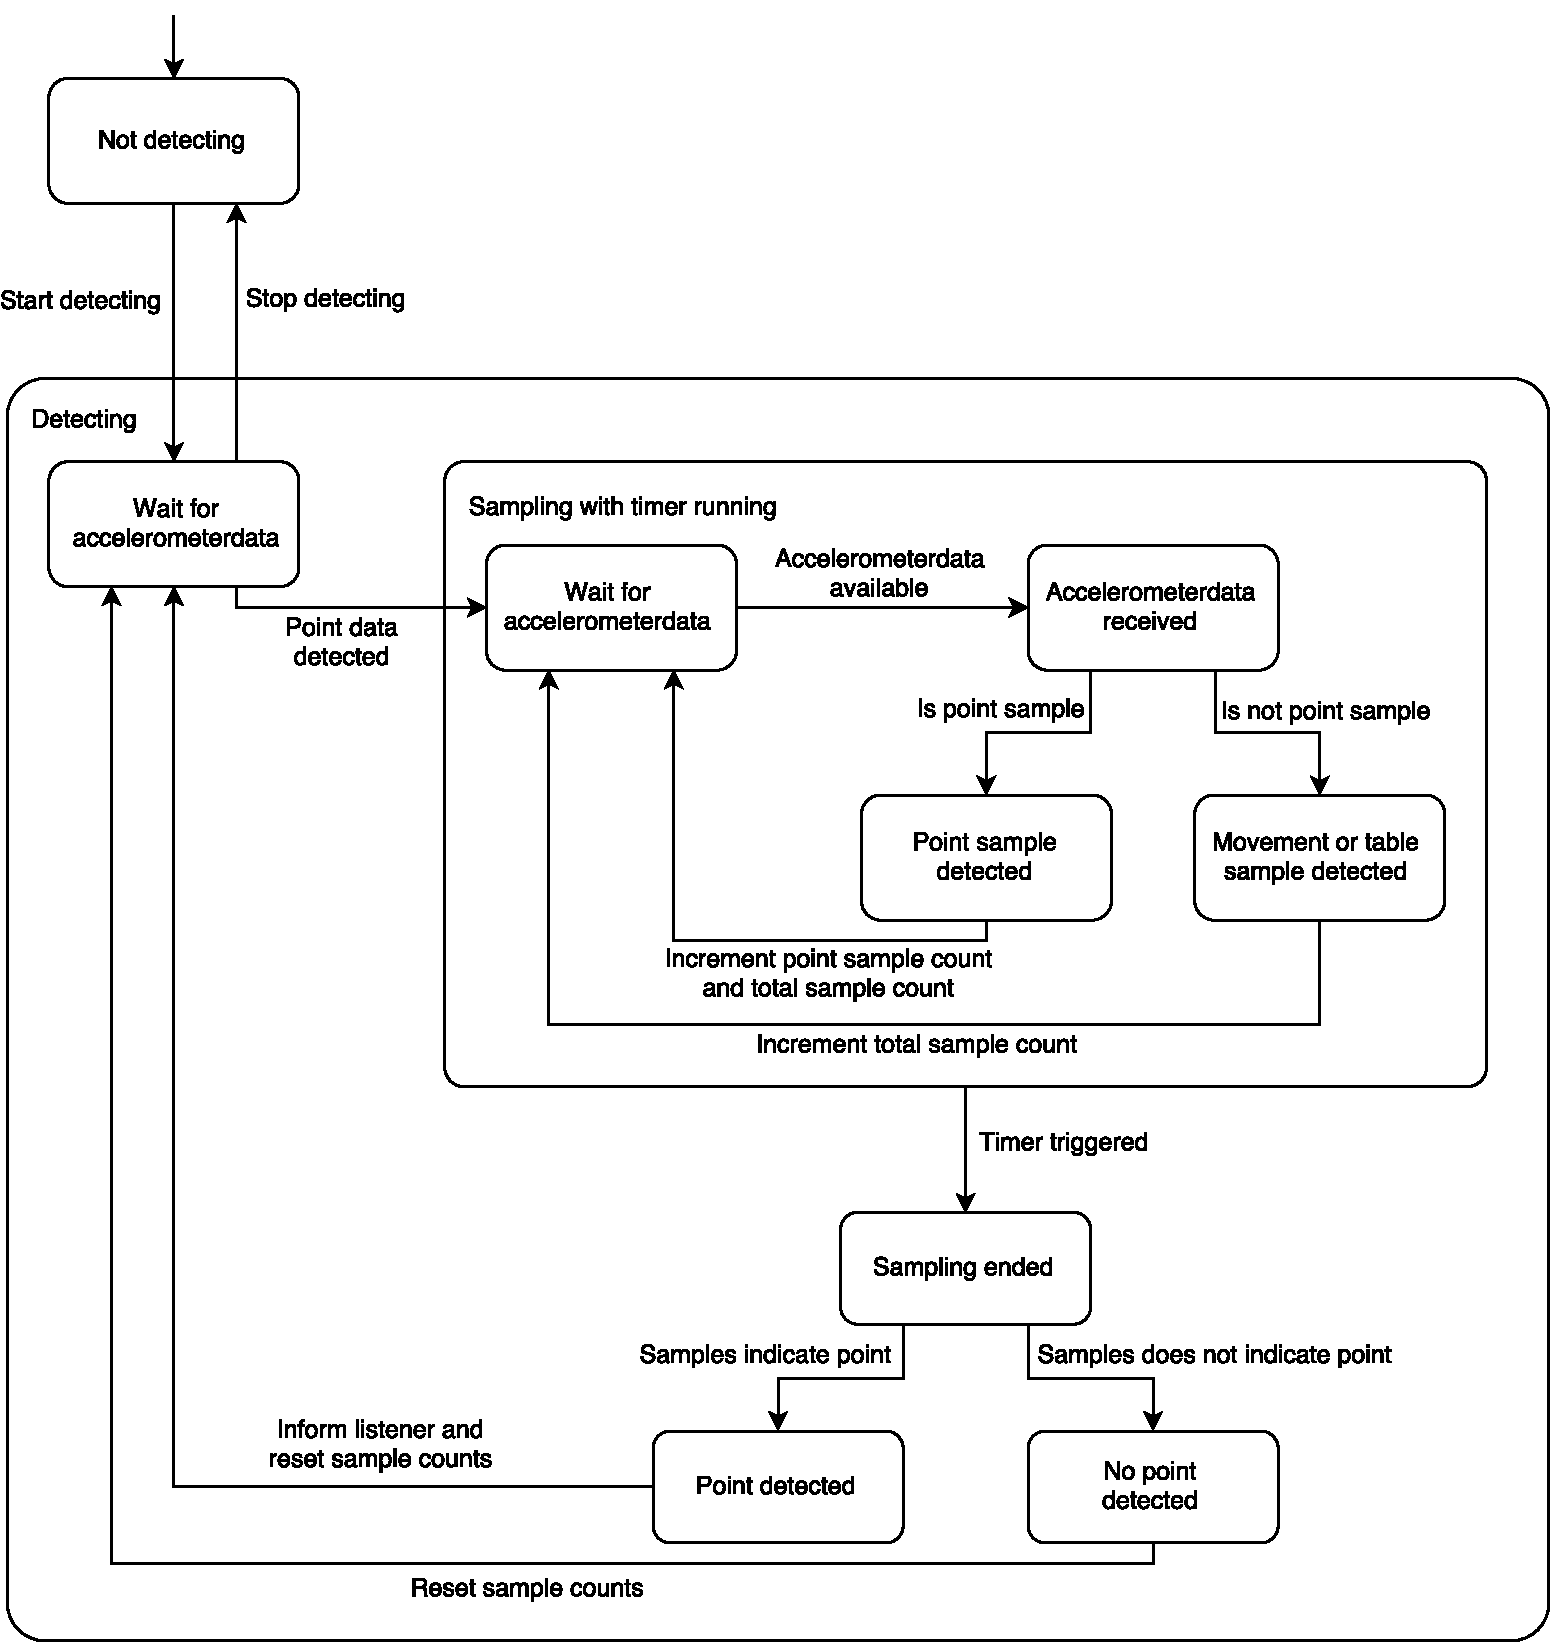
\includegraphics[width=\textwidth]{images/point-detector-state-diagram}
\caption{State diagram showing the states the \texttt{PointDetector} class can be in.}
\label{fig:gesture-recognition:pointdetector-state-diagram}
\end{figure}

The following pseudo code checks if a data set from the accelerometer indicates a point. 
\texttt{DataFitsWithinThreshold} takes the data from the accelerometer and a threshold $t$. \\
The function returns whether or not all of the $x$-, $y$- and $z$-values in the accelerometer data fits within the threshold.

\begin{algorithm}
  \begin{algorithmic}
    \Function{DataFitsWithinThreshold}{$data$, $t$}
      \State \Return $data.x \leq t \And data.x \geq -t \And data.y \leq t \And data.y \geq -t \And data.z \leq t \And data.z \geq -t$
    \EndFunction
  \end{algorithmic}
\end{algorithm}

The function \texttt{AccelerometerDataIndicatesPoint} takes data from the accelerometer data, 
and checks if the data fits within the threshold $g$, 
indicating that the data comes from a device lying on the table. 
If the data fits within $g$, 
the function returns false. 
%Thalley: Jeg kan overhovedet ikke læse og forstå den næste sætning :s
If not, the functions returns whether or not the data fits within the threshold $h$, 
some small number specifying a approximate of the acceleration given to the device when pointed with.

\begin{algorithm}
  \begin{algorithmic}
    \Function{AccelerometerDataIndicatesPoint}{$data$}
    \If{\Call{DataFitsWithinThreshold}{data, g}}
    \State \Return \texttt{false}
    \Else
    \State \Return \Call{DataFitsWithinThreshold}{data, h}
    \EndIf
    \EndFunction
  \end{algorithmic}
\end{algorithm}

\Cref{fig:gesture-recognition:pointdetector-uml} shows an example of the attributes and operations the \texttt{PointDetector} may have. 
Most of the attributes and operations should be self-explanatory but some may need a short description.

\begin{itemize}
  \item \texttt{pointingDuration} specifies the duration of the timer registered when entering the sampling phase.
  \item \texttt{pointingSampleFrequency} corresponds to $c$, the percentage of samples that must indicate a point.
  \item \texttt{pointingThreshold} corresponds to $h$, the threshold of data when determining if the device is lying on the table.
  \item \texttt{tableThreshold} corresponds to $g$, the threshold of data when determining if the device is being pointed with.
  \item \texttt{pointDetectedCallback} is a closure called when a point is detected.
\end{itemize}

\begin{figure}
  \centering
  \begin{tikzpicture} 
    \umlclass[x=0,y=0]{PointDetector}{
    +/- isDetecting: Bool\\
    - isSampling: Bool\\
    - pointingDuration: Float\\
    - pointingSampleFrequency: Float\\
    - pointingThreshold: Float\\
    - tableThreshold: Float\\
    - samplingTimer: Timer\\
    - pointingSampleCount: Int\\
    - totalSampleCount: Int\\
    - pointDetectedCallback: Closure
    }{
    + beginDetecting()\\
    + endDetecting()\\
    - didReceiveAccelerometerData(data: AccelerometerData)\\
    - accelerometerDataIndicatesPoint(data: AccelerometerData): Bool\\
    - dataFitsWithinThreshold(data: AccelerometerData, threshold: Double): Bool\\
    - samplingTimerTriggered()
    } 
  \end{tikzpicture}
  \caption{Class diagram of the \texttt{PointDetector} class.}
  \label{fig:gesture-recognition:pointdetector-uml}
\end{figure}

%%% Local Variables:
%%% mode: latex
%%% TeX-master: "../../master"
%%% TeX-command-extra-options: "-shell-escape"
%%% End:
